\documentclass{article}

% content/resources/templates/preamble.tex
\usepackage[margin=0.6in]{geometry}
\author{Milav Dabgar}
\usepackage{amsmath,amssymb,amsthm}
\usepackage{booktabs}
\usepackage{multirow}
\usepackage{xcolor}
\usepackage{tcolorbox}
\tcbuselibrary{breakable,skins}
\usepackage[colorlinks=true,linkcolor=blue]{hyperref}
\usepackage{titlesec}
\usepackage{enumitem}
\usepackage{tikz}
\usepackage{pgfplots}
\usepackage{circuitikz}
\usepackage[version=4]{mhchem}
\usepackage{longtable}
\usepackage{array}
\usepackage{float}
\usepackage{caption}
\usepackage{listings}

\lstset{
  basicstyle=\small\ttfamily,
  breaklines=true,
  breakatwhitespace=false,
  postbreak=\mbox{\textcolor{red}{$\hookrightarrow$}\space},
  float=false,
  numbers=left,
  numberstyle=\tiny\color{gray},
  numbersep=10pt,
  xleftmargin=2em,
  keywordstyle=\color{blue},
  commentstyle=\color{green!60!black},
  stringstyle=\color{purple},
  backgroundcolor=\color{gray!5},
  showstringspaces=false,
  tabsize=2,
  captionpos=b,
  keepspaces=true,
  columns=flexible
}

\pgfplotsset{compat=1.18}
\usetikzlibrary{shapes,arrows,positioning,calc,patterns,decorations.pathmorphing,decorations.markings,arrows.meta}

% Color scheme
\definecolor{headcolor}{RGB}{0,102,204}
\definecolor{keycolor}{RGB}{220,20,60}
\definecolor{solutioncolor}{RGB}{34,139,34}
\definecolor{mnemoniccolor}{RGB}{148,0,211}
\definecolor{codecolor}{RGB}{0,0,100}

% Spacing
\setlength{\parskip}{3pt}
\setlist[itemize]{nosep}
\setlist[enumerate]{nosep}

% Title formatting
\titleformat{\section}{\Large\bfseries\color{headcolor}}{\thesection}{1em}{}
\titleformat{\subsection}{\large\bfseries\color{headcolor}}{\thesubsection}{1em}{}

% Pandoc tightlist compatibility
\providecommand{\tightlist}{%
  \setlength{\itemsep}{0pt}\setlength{\parskip}{0pt}}

% Pandoc longtable compatibility
\newcounter{none}
\def\thenone{}


% content/resources/templates/english-boxes.tex

% Custom environments
\newtcolorbox{solutionbox}{
 breakable,
 enhanced,
 colback=solutioncolor!5!white,
 colframe=solutioncolor!75!black,
 fonttitle=\bfseries,
 title=Solution
}

\newtcolorbox{solutionboxnobreak}{
 colback=solutioncolor!5!white,
 colframe=solutioncolor!75!black,
 fonttitle=\bfseries,
 title=Solution
}

\newtcolorbox{keyformula}{
 breakable,
 enhanced,
 colback=keycolor!5!white,
 colframe=keycolor!75!black,
 fonttitle=\bfseries,
 title=Key Formula
}

\newtcolorbox{mnemonicboxenv}{
 breakable,
 enhanced,
 colback=mnemoniccolor!5!white,
 colframe=mnemoniccolor!75!black,
 fonttitle=\bfseries,
 title=Mnemonic
}

\newcommand{\mnemonicbox}[1]{%
  \begin{mnemonicboxenv}
    #1
  \end{mnemonicboxenv}
}


% Custom commands for GTU solutions
% This file defines semantic commands for consistent formatting

% Question command with automatic formatting
\newcommand{\question}[2]{%
  \section*{Question #1}%
  \textbf{#2}%
}

% OR question variant
\newcommand{\questionor}[2]{%
  \section*{Question #1 OR}%
  \textbf{#2}%
}

% Proper table environment with caption
\newenvironment{answertable}[1]{%
  \begin{table}[htbp]
  \centering
  \caption{#1}
}{%
  \end{table}
}

% Proper figure environment for diagrams
\newenvironment{answerdiagram}[1]{%
  \begin{figure}[htbp]
  \centering
  \caption{#1}
}{%
  \end{figure}
}

% Semantic markup for key terms
\newcommand{\keyword}[1]{\textbf{#1}}
\newcommand{\code}[1]{\texttt{#1}}
\newcommand{\classname}[1]{\texttt{#1}}
\newcommand{\methodname}[1]{\texttt{#1}}

% Proper quotation marks
\newcommand{\mnemonic}[1]{``#1''}


\title{Industrial Electronics (4331103) - Winter 2022 Solution}
\date{March 1, 2023}

\begin{document}
\maketitle

\questionmarks{1(a)}{3}{Draw the construction of SCR and explain it.}

\begin{solutionbox}
SCR (Silicon Controlled Rectifier) is a four-layer PNPN semiconductor device with three terminals: Anode, Cathode, and Gate.

\begin{center}
\begin{tikzpicture}[auto, node distance=1.5cm]
    \node [gtu block, minimum width=2cm, fill=blue!10] (P1) {P};
    \node [gtu block, minimum width=2cm, fill=red!10, below=0cm of P1] (N1) {N};
    \node [gtu block, minimum width=2cm, fill=blue!10, below=0cm of N1] (P2) {P};
    \node [gtu block, minimum width=2cm, fill=red!10, below=0cm of P2] (N2) {N};
    
    \draw [thick] (P1.north) -- ++(0,0.5) node[above] {Anode (A)};
    \draw [thick] (N2.south) -- ++(0,-0.5) node[below] {Cathode (K)};
    \draw [thick] (P2.east) -- ++(0.5,0) node[right] {Gate (G)};
\end{tikzpicture}
\captionof{figure}{SCR Construction}
\end{center}

\begin{itemize}
    \item \keyword{P-N-P-N Layers}: Four alternating semiconductor layers.
    \item \keyword{Gate Terminal}: Controls turn-on of the device.
    \item \keyword{Current Flow}: Anode to cathode when triggered.
\end{itemize}
\end{solutionbox}

\begin{mnemonicbox}
\mnemonic{Silicon Controls Rectification: SCR controls current flow in one direction only when triggered.}
\end{mnemonicbox}

\questionmarks{1(b)}{4}{Draw construction of TRIAC and explain it.}

\begin{solutionbox}
TRIAC (Triode for Alternating Current) is a bidirectional three-terminal semiconductor device that conducts in both directions when triggered.

\begin{center}
\begin{tikzpicture}[auto, node distance=0cm]
    \node [gtu block, minimum width=2.5cm, fill=red!10] (N4) {N4};
    \node [gtu block, minimum width=3cm, fill=blue!10, below=0cm of N4] (P1) {P1};
    \node [gtu block, minimum width=3cm, fill=red!10, below=0cm of P1] (N1) {N1};
    \node [gtu block, minimum width=3cm, fill=blue!10, below=0cm of N1] (P2) {P2};
    \node [gtu block, minimum width=1.5cm, fill=red!10, below=0cm of P2, xshift=-0.75cm] (N2) {N2};
    \node [gtu block, minimum width=1.5cm, fill=red!10, below=0cm of P2, xshift=0.75cm] (N3) {N3};
    
    \draw [thick] (P1.north) -- ++(0,0.5) node[above] {MT1};
    \draw [thick] (P2.south) -- ++(0,-0.5) node[below] {MT2};
    \draw [thick] (P2.east) -- ++(0.5,0) node[right] {Gate (G)};
\end{tikzpicture}
\captionof{figure}{TRIAC Construction}
\end{center}

\begin{itemize}
    \item \keyword{Bidirectional Operation}: Conducts in both directions when triggered.
    \item \keyword{Gate Control}: Single gate controls conduction in both directions.
    \item \keyword{Equivalent Circuit}: Acts like two SCRs connected in anti-parallel.
    \item \keyword{AC Applications}: Widely used for AC power control applications.
\end{itemize}
\end{solutionbox}

\begin{mnemonicbox}
\mnemonic{TRI-direction AC controller: Controls current in both directions in AC circuits.}
\end{mnemonicbox}

\questionmarks{1(c)}{7}{Describe construction \& working of Opto-Isolators, Opto-TRIAC, Opto-SCR, and Opto-transistor. And list their applications.}

\begin{solutionbox}
Opto-isolators use light to transfer electrical signals between isolated circuits.

\begin{center}
\begin{tikzpicture}[auto, node distance=2cm]
    \node [gtu block, fill=yellow!10] (LED) {LED};
    \node [gtu block, right=of LED, fill=green!10] (PD) {Photo Detector};
    
    \draw [gtu arrow, dashed] (LED) -- node {Light} (PD);
    
    \node [left=0.5cm of LED] (Input) {Input};
    \node [right=0.5cm of PD] (Output) {Output};
    
    \draw [thick] (Input) -- (LED);
    \draw [thick] (PD) -- (Output);
\end{tikzpicture}
\captionof{figure}{Basic Opto-Isolator Block Diagram}
\end{center}

\begin{center}
\captionof{table}{Opto-Isolator Types and Applications}
\begin{tabulary}{\linewidth}{|L|L|L|L|}
\hline
\textbf{Device} & \textbf{Construction} & \textbf{Working} & \textbf{Applications} \\ \hline
Opto-Isolator & LED + Photodetector & LED emits light when input current flows; photodetector activates output circuit & Signal isolation, Medical equipment, Industrial controls \\ \hline
Opto-TRIAC & LED + Photo-TRIAC & LED triggers the TRIAC through light; provides electrical isolation & AC power control, Solid state relays, Motor controls \\ \hline
Opto-SCR & LED + Photo-SCR & LED emits light to trigger SCR; provides high isolation & DC switching, Industrial controls, High voltage isolation \\ \hline
Opto-transistor & LED + Photo-transistor & LED light controls base current of phototransistor & Encoders, Level detection, Position sensing \\ \hline
\end{tabulary}
\end{center}

\begin{itemize}
    \item \keyword{Electrical Isolation}: Complete separation between input and output.
    \item \keyword{Noise Immunity}: High resistance to electrical noise.
    \item \keyword{Speed}: Response times in microseconds range.
\end{itemize}
\end{solutionbox}

\begin{mnemonicbox}
\mnemonic{LOST: Light Operates Semiconductor Terminals in all opto-devices.}
\end{mnemonicbox}

\questionmarks{1(c OR)}{7}{Describe Explain working of SCR using two transistor analogies. List the various industrial applications of SCR.}

\begin{solutionbox}
SCR can be modeled as two interconnected transistors: PNP (T1) and NPN (T2).

\begin{center}
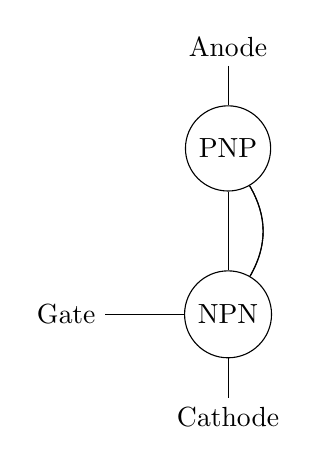
\begin{tikzpicture}[auto, node distance=2cm]
    \node (A) {Anode};
    \node [draw, circle, below=0.5cm of A] (T1) {PNP};
    \node [draw, circle, below=1cm of T1] (T2) {NPN};
    \node [below=0.5cm of T2] (K) {Cathode};
    \node [left=1cm of T2] (G) {Gate};
    
    \draw (A) -- (T1);
    \draw (T1) -- (T2);
    \draw (T2) -- (K);
    \draw (G) -- (T2);
    \draw (T1) to[bend left] (T2); % Collector T1 to Base T2
    \draw (T2) to[bend right] (T1); % Collector T2 to Base T1
\end{tikzpicture}
\captionof{figure}{Two Transistor Analogy of SCR}
\end{center}

\textbf{Working Principle:}

\begin{center}
\begin{tabulary}{\linewidth}{|L|L|}
\hline
\textbf{Step} & \textbf{Operation} \\ \hline
Initial State & Both transistors are OFF \\ \hline
Gate Triggering & Current injected into gate (B2 of T2) \\ \hline
Regenerative Action & T2 turns ON $\to$ T1 base gets current $\to$ T1 turns ON $\to$ More current to T2 base \\ \hline
Latching & Self-sustaining current flow continues even if gate signal is removed \\ \hline
\end{tabulary}
\end{center}

\textbf{Industrial Applications of SCR:}
\begin{itemize}
    \item \keyword{Power Control}: AC/DC motor speed control.
    \item \keyword{Switching}: Static switches, solid-state relays.
    \item \keyword{Inverters}: DC to AC conversion.
    \item \keyword{Protection}: Overvoltage protection circuits.
    \item \keyword{Lighting}: Light dimmers, illumination control.
\end{itemize}
\end{solutionbox}

\begin{mnemonicbox}
\mnemonic{POWER: Power control, Overvoltage protection, Welding machines, Electronic converters, Regulated supplies.}
\end{mnemonicbox}

\questionmarks{2(a)}{3}{Define Triggering in SCR and explain any two triggering techniques.}

\begin{solutionbox}
Triggering is the process of turning ON an SCR by applying appropriate signal to its gate terminal.

\textbf{Two Triggering Techniques:}

\begin{center}
\captionof{table}{Triggering Techniques}
\begin{tabulary}{\linewidth}{|L|L|}
\hline
\textbf{Technique} & \textbf{Description} \\ \hline
Gate Triggering & Direct current pulse applied to gate-cathode circuit \\ \hline
Light Triggering & Photons striking junction provide energy for conduction \\ \hline
\end{tabulary}
\end{center}

\begin{itemize}
    \item \keyword{Gate Triggering}: Most common method using electrical pulse.
    \item \keyword{Light Triggering}: Uses photosensitive semiconductor properties.
\end{itemize}
\end{solutionbox}

\begin{mnemonicbox}
\mnemonic{GET: Gate Electrical Triggering is the most common method.}
\end{mnemonicbox}

\questionmarks{2(b)}{4}{Write the differences between forced commutation and natural commutation.}

\begin{solutionbox}
\begin{center}
\captionof{table}{Forced vs Natural Commutation}
\begin{tabulary}{\linewidth}{|L|L|L|}
\hline
\textbf{Parameter} & \textbf{Forced Commutation} & \textbf{Natural Commutation} \\ \hline
Definition & External circuitry forces SCR to turn OFF & SCR turns OFF naturally when current falls below holding value \\ \hline
Application & DC circuits & AC circuits \\ \hline
Components & Requires additional components (capacitors, inductors) & No additional components needed \\ \hline
Complexity & Complex circuit design & Simple circuit design \\ \hline
Energy & External energy needed for turn-off & No external energy needed \\ \hline
\end{tabulary}
\end{center}

\begin{itemize}
    \item \keyword{Forced Commutation}: Actively turns OFF SCR using external circuit.
    \item \keyword{Natural Commutation}: SCR turns OFF when AC current crosses zero.
\end{itemize}
\end{solutionbox}

\begin{mnemonicbox}
\mnemonic{FACE: Forced Active Commutation requires External components.}
\end{mnemonicbox}

\questionmarks{2(c)}{7}{Design the snubber circuit for SCR.}

\begin{solutionbox}
Snubber circuit protects SCR from high $dV/dt$ and limits rate of voltage rise.

\begin{center}
\begin{tikzpicture}[auto, node distance=2cm]
    \node (A) [label=above:Anode] {};
    \node (K) [label=below:Cathode, below=3cm of A] {};
    \node [gtu block, minimum width=1cm, minimum height=1.5cm] (SCR) at ($(A)!0.5!(K)$) {SCR};
    
    \draw (A) -- (SCR);
    \draw (SCR) -- (K);
    
    % Snubber branch
    \draw (A) -- ++(2,0) coordinate (B);
    \draw (B) to[R, l=$R_s$] ++(0,-1.5) coordinate (C);
    \draw (C) to[C, l=$C_s$] ++(0,-1.5) coordinate (D);
    \draw (D) -- (K);
\end{tikzpicture}
\captionof{figure}{RC Snubber Circuit}
\end{center}

\textbf{Design Steps:}

\begin{center}
\begin{tabulary}{\linewidth}{|L|L|}
\hline
\textbf{Step} & \textbf{Calculation} \\ \hline
1. Calculate $dV/dt$ rating & From datasheet (V/$\mu$s) \\ \hline
2. Determine $R$ value & $R = V_1/I_L$ where $V_1$ is supply voltage and $I_L$ is load current \\ \hline
3. Determine $C$ value & $C = 1/(R \times (dV/dt)_{max})$ \\ \hline
4. RC time constant & $\tau = R \times C$ (should be greater than SCR turn-off time) \\ \hline
\end{tabulary}
\end{center}

\begin{itemize}
    \item \keyword{Resistance R}: Limits discharge current of capacitor.
    \item \keyword{Capacitance C}: Absorbs transient energy and limits $dV/dt$.
    \item \keyword{Protection}: Prevents false triggering and damage.
    \item \keyword{Power Rating}: R must have sufficient power rating.
\end{itemize}
\end{solutionbox}

\begin{mnemonicbox}
\mnemonic{RCSS: Resistance-Capacitance Saves Silicon from Stress.}
\end{mnemonicbox}

\questionmarks{2(a OR)}{3}{Define commutation and Explain class-E commutation for SCR.}

\begin{solutionbox}
Commutation is the process of turning OFF an SCR by reducing its anode current below the holding current level.

\textbf{Class-E Commutation:}

\begin{center}
\begin{tikzpicture}[auto, node distance=2cm]
    \node (S) {Supply};
    \node [gtu block, right=of S] (L) {Load};
    \node [gtu block, right=of L, label=below:Main SCR] (SCR) {SCR};
    \node [gtu block, below=of L] (C) {Capacitor};
    \node [gtu block, below=of C, label=below:Aux SCR] (A) {Aux SCR};
    
    \draw [thick] (S) -- (L);
    \draw [thick] (L) -- (SCR);
    \draw [thick] (L) -- (C);
    \draw [thick] (C) -- (A);
    \draw [thick] (A) -| (S);
\end{tikzpicture}
\captionof{figure}{Class-E Commutation Circuit (Conceptual)}
\end{center}

\begin{itemize}
    \item \keyword{Auxiliary SCR}: Controls the commutation process.
    \item \keyword{Resonant Circuit}: Forms LC resonant circuit.
    \item \keyword{Operation}: Auxiliary SCR triggers capacitor discharge to reverse-bias main SCR.
    \item \keyword{Application}: Used in inverters and choppers.
\end{itemize}
\end{solutionbox}

\begin{mnemonicbox}
\mnemonic{ACE: Auxiliary Capacitor Extinguishes conduction.}
\end{mnemonicbox}

\questionmarks{2(b OR)}{4}{Explain Triggering of Thyristor.}

\begin{solutionbox}
\begin{center}
\captionof{table}{Thyristor Triggering Methods}
\begin{tabulary}{\linewidth}{|L|L|}
\hline
\textbf{Triggering Method} & \textbf{Working Principle} \\ \hline
Gate Triggering & Electrical pulse applied between gate and cathode \\ \hline
Temperature Triggering & Junction temperature increases to cause turn-on \\ \hline
Light Triggering & Photons create electron-hole pairs at junctions \\ \hline
$dV/dt$ Triggering & Rapid voltage rise causes capacitive current flow \\ \hline
Forward Voltage Triggering & Exceeding breakover voltage causes avalanche conduction \\ \hline
\end{tabulary}
\end{center}

\begin{itemize}
    \item \keyword{Gate Triggering}: Most common and controllable method.
    \item \keyword{Parameter Control}: Pulse width, amplitude, and rise time.
    \item \keyword{Gate Sensitivity}: Varies with temperature.
    \item \keyword{Protection}: Required against unwanted triggering.
\end{itemize}
\end{solutionbox}

\begin{mnemonicbox}
\mnemonic{VITAL: Voltage, Illumination, Temperature And Level are all triggering methods.}
\end{mnemonicbox}

\questionmarks{2(c OR)}{7}{Explain methods to protect SCR against over voltage and current in details.}

\begin{solutionbox}
\textbf{Overvoltage Protection:}

\begin{center}
\begin{tikzpicture}[auto, node distance=1.5cm]
    \node (S) {Supply};
    \node [right=of S] (F) {Fuse};
    \node [right=of F] (J) {};
    \node [above=of J] (V) {Varistor};
    \node [right=of J] (SCR) {SCR};
    \node [right=of SCR] (L) {Load};
    \node [below=of J] (RC) {RC Snubber};
    
    \draw (S) -- (F) -- (J) -- (SCR) -- (L);
    \draw (J) -- (V);
    \draw (J) -- (RC);
\end{tikzpicture}
\captionof{figure}{Overvoltage Protection Scheme}
\end{center}

\begin{center}
\captionof{table}{Overvoltage Protection Methods}
\begin{tabulary}{\linewidth}{|L|L|}
\hline
\textbf{Protection Method} & \textbf{Working Principle} \\ \hline
RC Snubber Circuit & Limits rate of rise of voltage ($dV/dt$) \\ \hline
Voltage Clamping & Using Zener diodes or MOVs to limit maximum voltage \\ \hline
Crowbar Protection & Deliberate short-circuit when voltage exceeds threshold \\ \hline
\end{tabulary}
\end{center}

\textbf{Overcurrent Protection:}

\begin{center}
\captionof{table}{Overcurrent Protection Methods}
\begin{tabulary}{\linewidth}{|L|L|}
\hline
\textbf{Protection Method} & \textbf{Working Principle} \\ \hline
Fuses/Circuit Breakers & Disconnects circuit during fault conditions \\ \hline
Current Limiting Reactors & Limits fault current magnitude \\ \hline
Electronic Current Limiting & Sensing and control circuits limit current \\ \hline
\end{tabulary}
\end{center}

\begin{itemize}
    \item \keyword{Coordination}: Protection devices must work in coordination.
    \item \keyword{Response Time}: Critical for effective protection.
    \item \keyword{Multiple Layers}: For critical applications, several methods are combined.
\end{itemize}
\end{solutionbox}

\begin{mnemonicbox}
\mnemonic{SCOPE: Snubbers, Clamps, Overload sensors, Protectors, and Electronic limiters.}
\end{mnemonicbox}

\questionmarks{3(a)}{3}{List the differences between single phase rectifier and poly phase rectifier.}

\begin{solutionbox}
\begin{center}
\captionof{table}{Single Phase vs Poly Phase Rectifier}
\begin{tabulary}{\linewidth}{|L|L|L|}
\hline
\textbf{Parameter} & \textbf{Single Phase Rectifier} & \textbf{Poly Phase Rectifier} \\ \hline
Input & Single phase AC supply & Multiple phase (usually 3-phase) AC supply \\ \hline
Output Ripple & Higher ripple content & Lower ripple content \\ \hline
Efficiency & Lower efficiency & Higher efficiency \\ \hline
Power Rating & Suitable for low power applications & Suitable for high power applications \\ \hline
Transformer Utilization & Lower utilization factor & Higher utilization factor \\ \hline
\end{tabulary}
\end{center}

\begin{itemize}
    \item \keyword{Ripple Factor}: Single phase has higher ripple compared to poly phase.
    \item \keyword{Form Factor}: Better in poly phase systems.
    \item \keyword{Size/Weight}: Poly phase systems have better power/weight ratio.
\end{itemize}
\end{solutionbox}

\begin{mnemonicbox}
\mnemonic{PERCH: Poly phase has Efficiency, Ripple improvement, Capacity, and Higher ratings.}
\end{mnemonicbox}

\questionmarks{3(b)}{4}{Draw the circuit diagram of three phases Half Wave Rectifier and explain its Working.}

\begin{solutionbox}
Three-phase half-wave rectifier converts three-phase AC into pulsating DC using three diodes.

\begin{center}
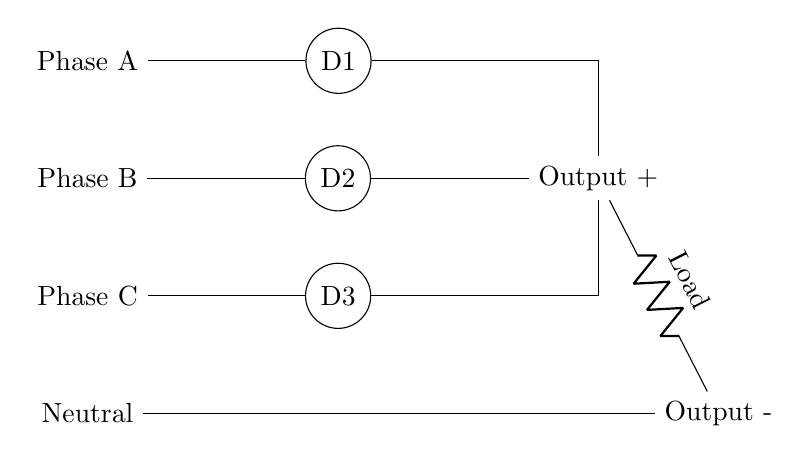
\begin{tikzpicture}[auto, node distance=1.5cm]
    \node (A) {Phase A};
    \node [below=1cm of A] (B) {Phase B};
    \node [below=1cm of B] (C) {Phase C};
    \node [below=1cm of C] (N) {Neutral};
    
    \node [right=2cm of A, draw, circle] (D1) {D1};
    \node [right=2cm of B, draw, circle] (D2) {D2};
    \node [right=2cm of C, draw, circle] (D3) {D3};
    
    \draw (A) -- (D1);
    \draw (B) -- (D2);
    \draw (C) -- (D3);
    
    \node [right=2cm of D2] (O) {Output +};
    \node [right=6.5cm of N] (ON) {Output -};
    
    \draw (D1) -| (O);
    \draw (D2) -- (O);
    \draw (D3) -| (O);
    \draw (N) -- (ON);
    
    \draw (O) to[R, l=Load] (ON);
\end{tikzpicture}
\captionof{figure}{3-Phase Half Wave Rectifier}
\end{center}

\textbf{Working:}
\begin{itemize}
    \item Each diode conducts when its phase voltage is most positive.
    \item Conduction angle of each diode is $120^\circ$.
    \item Ripple frequency is 3 times the input frequency.
    \item Average output voltage = $3V_m/2\pi$ (where $V_m$ is peak phase voltage).
    \item Ripple factor = 0.17 (much lower than single-phase half-wave).
\end{itemize}
\end{solutionbox}

\begin{mnemonicbox}
\mnemonic{THREE-D: THREE Diodes conducting sequentially.}
\end{mnemonicbox}

\questionmarks{3(c)}{7}{Describe the working of UPS \& SMPS with the help of block diagram.}

\begin{solutionbox}
\textbf{UPS (Uninterruptible Power Supply):}

\begin{center}
\begin{tikzpicture}[auto, node distance=1.5cm]
    \node [gtu block] (R) {Rectifier};
    \node [gtu block, right=of R] (B) {Battery};
    \node [gtu block, right=of B] (I) {Inverter};
    \node [gtu block, right=of I] (F) {Filter};
    \node [left=of R] (AC) {AC Input};
    \node [right=of F] (L) {Load};
    
    \draw [gtu arrow] (AC) -- (R);
    \draw [gtu arrow] (R) -- (B);
    \draw [gtu arrow] (B) -- (I);
    \draw [gtu arrow] (I) -- (F);
    \draw [gtu arrow] (F) -- (L);
    \draw [gtu arrow, dashed] (AC) to[bend left] node {Bypass} (L);
\end{tikzpicture}
\captionof{figure}{UPS Block Diagram}
\end{center}

\begin{center}
\captionof{table}{UPS Blocks and Functions}
\begin{tabulary}{\linewidth}{|L|L|}
\hline
\textbf{Block} & \textbf{Function} \\ \hline
Rectifier & Converts AC to DC for battery charging and inverter \\ \hline
Battery & Stores energy for backup during power failure \\ \hline
Inverter & Converts DC to AC for powering load \\ \hline
Filter & Smooths output waveform \\ \hline
Bypass & Provides direct AC during maintenance \\ \hline
\end{tabulary}
\end{center}

\textbf{SMPS (Switched Mode Power Supply):}

\begin{center}
\begin{tikzpicture}[auto, node distance=1.2cm]
    \node [gtu block] (RF1) {Rectifier \& Filter};
    \node [gtu block, right=of RF1] (SW) {Switch};
    \node [gtu block, right=of SW] (T) {Transformer};
    \node [gtu block, right=of T] (RF2) {Rectif/Filter};
    \node [below=of SW] (FB) {Feedback};
    \node [left=of RF1] (AC) {AC In};
    \node [right=of RF2] (DC) {DC Out};

    \draw [gtu arrow] (AC) -- (RF1);
    \draw [gtu arrow] (RF1) -- (SW);
    \draw [gtu arrow] (SW) -- (T);
    \draw [gtu arrow] (T) -- (RF2);
    \draw [gtu arrow] (RF2) -- (DC);
    \draw [gtu arrow] (RF2) |- (FB);
    \draw [gtu arrow] (FB) -- (SW);
\end{tikzpicture}
\captionof{figure}{SMPS Block Diagram}
\end{center}

\begin{itemize}
    \item \keyword{UPS Efficiency}: 80-90\%, provides backup power.
    \item \keyword{SMPS Efficiency}: 70-90\%, much smaller than linear supplies.
    \item \keyword{Regulation}: Both provide regulated output voltage.
\end{itemize}
\end{solutionbox}

\begin{mnemonicbox}
\mnemonic{BRIEF: Battery backup, Rectification, Inversion, Efficient switching, Feedback control.}
\end{mnemonicbox}

\questionmarks{3(a OR)}{3}{Explain the Principle \& working of Chopper circuits.}

\begin{solutionbox}
Chopper is a DC-to-DC converter that converts fixed DC input voltage to variable DC output voltage.

\begin{center}
\begin{tikzpicture}[auto, node distance=2cm]
    \node (DC) {DC Source};
    \node [gtu block, right=of DC] (S) {Switch/SCR};
    \node [gtu block, right=of S] (L) {Load};
    
    \draw [thick] (DC) -- (S);
    \draw [thick] (S) -- (L);
    \draw [thick] (L.south) -- ++(0,-0.5) -| (DC.south);
\end{tikzpicture}
\captionof{figure}{Basic Chopper Circuit}
\end{center}

\textbf{Principle:}
\begin{itemize}
    \item Switch (typically SCR, MOSFET, or IGBT) rapidly connects and disconnects source to load.
    \item Output voltage controlled by duty cycle (ON time / total time).
    \item Average output voltage = Input voltage $\times$ Duty cycle.
    \item \keyword{Time Ratio Control}: Varies duty cycle, keeping frequency constant.
    \item \keyword{Frequency Modulation}: Varies frequency, keeping ON time constant.
\end{itemize}
\end{solutionbox}

\begin{mnemonicbox}
\mnemonic{CHOP: Control High-speed Operation with Pulses.}
\end{mnemonicbox}

\questionmarks{3(b OR)}{4}{Compare single-phase and Poly-phase rectifier circuits.}

\begin{solutionbox}
\begin{center}
\captionof{table}{Single-Phase vs Poly-Phase Rectifier}
\begin{tabulary}{\linewidth}{|L|L|L|}
\hline
\textbf{Parameter} & \textbf{Single-Phase Rectifier} & \textbf{Poly-Phase Rectifier} \\ \hline
Supply & Single-phase AC & Three or more phase AC \\ \hline
Output Waveform & More pulsating & Smoother (less pulsating) \\ \hline
Ripple Content & Higher (0.48 for full wave) & Lower (0.042 for 3-phase full wave) \\ \hline
Filtering & More filtering required & Less filtering required \\ \hline
Power Handling & Limited power handling & Higher power handling \\ \hline
Transformer Utilization & 0.812 (full wave) & 0.955 (3-phase full wave) \\ \hline
Efficiency & Lower & Higher \\ \hline
Size & Smaller for same power & More compact for high power \\ \hline
\end{tabulary}
\end{center}

\begin{itemize}
    \item \keyword{Harmonic Content}: Lower in poly-phase systems.
    \item \keyword{TUF}: Higher in poly-phase systems.
    \item \keyword{Cost-Effectiveness}: Poly-phase more economical for high power.
\end{itemize}
\end{solutionbox}

\begin{mnemonicbox}
\mnemonic{PERIPHERY: Poly-phase Efficiency Ripple Improvement Power Handling Economy Rating Yield.}
\end{mnemonicbox}

\questionmarks{3(c OR)}{7}{Describe the working of solar Photovoltaic (PV) based power generation with the help of block diagram.}

\begin{solutionbox}
Solar PV power generation converts sunlight directly into electricity using semiconductor materials.

\begin{center}
\begin{tikzpicture}[auto, node distance=1.5cm]
    \node [draw, circle, fill=yellow!20] (Sun) {Sun};
    \node [gtu block, right=of Sun] (PV) {PV Array};
    \node [gtu block, right=of PV] (CC) {Charge Ctrl};
    \node [gtu block, right=of CC] (B) {Battery};
    \node [gtu block, below=of B] (I) {Inverter};
    \node [right=of I] (L) {AC Load};
    \node [below=of CC] (DCL) {DC Load};
    
    \draw [gtu arrow, dashed] (Sun) -- (PV);
    \draw [gtu arrow] (PV) -- (CC);
    \draw [gtu arrow] (CC) -- (B);
    \draw [gtu arrow] (B) -- (I);
    \draw [gtu arrow] (I) -- (L);
    \draw [gtu arrow] (CC) -- (DCL);
\end{tikzpicture}
\captionof{figure}{Solar PV Power Generation Block Diagram}
\end{center}

\begin{center}
\captionof{table}{PV System Components}
\begin{tabulary}{\linewidth}{|L|L|}
\hline
\textbf{Component} & \textbf{Function} \\ \hline
PV Array & Converts solar energy to DC electricity through photovoltaic effect \\ \hline
Charge Controller & Regulates battery charging and prevents overcharging \\ \hline
Battery Bank & Stores energy for use during night or cloudy conditions \\ \hline
Inverter & Converts DC to AC for powering AC loads \\ \hline
Grid Connection & Optional connection for feeding excess power to grid \\ \hline
\end{tabulary}
\end{center}

\begin{itemize}
    \item \keyword{Photovoltaic Effect}: Photons from sunlight knock electrons free in semiconductor.
    \item \keyword{Efficiency}: Typically 15-22\% for commercial panels.
\end{itemize}
\end{solutionbox}

\begin{mnemonicbox}
\mnemonic{SOLAR: Semiconductors Oriented Light-to-electricity Array Regulation.}
\end{mnemonicbox}

\questionmarks{4(a)}{3}{List the advantages of static switch.}

\begin{solutionbox}
\begin{center}
\captionof{table}{Advantages of Static Switch}
\begin{tabulary}{\linewidth}{|L|}
\hline
\textbf{Features} \\ \hline
No moving parts - higher reliability \\ \hline
Silent operation \\ \hline
Fast switching response (microseconds) \\ \hline
Longer operational life \\ \hline
No contact bounce or arcing \\ \hline
Compact size \\ \hline
Compatible with digital control systems \\ \hline
Lower maintenance requirements \\ \hline
\end{tabulary}
\end{center}

\begin{itemize}
    \item \keyword{Reliability}: No mechanical wear and tear.
    \item \keyword{Speed}: Much faster than mechanical switches.
    \item \keyword{Isolation}: Can provide electrical isolation.
\end{itemize}
\end{solutionbox}

\begin{mnemonicbox}
\mnemonic{SAFE: Speed, Arc-free, Fast response, Endurance.}
\end{mnemonicbox}

\questionmarks{4(b)}{4}{Draw the circuit diagram of A.C. Power control using DIAC-TRIAC and Explain it.}

\begin{solutionbox}
DIAC-TRIAC circuit provides smooth AC power control for resistive and inductive loads.

\begin{center}
\begin{tikzpicture}[auto, node distance=2cm]
    \node (AC) {AC Supply};
    \node [right=of AC] (L) {Load};
    \node [right=of L, draw] (TRIAC) {TRIAC};
    \node [below=of TRIAC] (G) {Gate};
    \node [left=of G] (DIAC) {DIAC};
    \node [left=of DIAC] (C) {C};
    \node [above=of C] (R2) {Var R};
    \node [above=of R2] (R1) {R1};
    
    \draw (AC) -- (L) -- (TRIAC.north);
    \draw (TRIAC.south) |- (AC);
    \draw (TRIAC.south) -- (G);
    \draw (G) -- (DIAC);
    \draw (DIAC) -- (C);
    \draw (C) -- (R2) -- (R1) -- (L);
\end{tikzpicture}
\captionof{figure}{DIAC-TRIAC Phase Control}
\end{center}

\textbf{Working:}
\begin{itemize}
    \item Variable resistor R2 controls charging rate of capacitor C.
    \item When capacitor voltage reaches DIAC breakover voltage, DIAC conducts.
    \item DIAC delivers trigger pulse to TRIAC gate.
    \item TRIAC conducts for remainder of half-cycle.
    \item \keyword{Phase Control}: Controls power by varying firing angle.
\end{itemize}
\end{solutionbox}

\begin{mnemonicbox}
\mnemonic{DIRECT: DIAC Initiates Regulated Energy Control in TRIAC.}
\end{mnemonicbox}

\questionmarks{4(c)}{7}{Describe function of DC power control circuit using SCR with UJT in triggering circuit.}

\begin{solutionbox}
UJT-triggered SCR circuit provides precise control of DC power to the load.

\begin{center}
\begin{tikzpicture}[auto, node distance=2cm]
    \node (DC) {DC};
    \node [right=of DC] (L) {Load};
    \node [right=of L] (SCR) {SCR};
    \node [below=of SCR] (G) {Gate};
    \node [left=of G] (R4) {R4};
    \node [above=of R4] (UJT) {UJT};
    \node [left=of UJT] (C) {C};
    \node [above=of C] (R2) {Var R};
    
    \draw (DC) -- (L) -- (SCR.north);
    \draw (SCR.south) |- (DC);
    \draw (UJT) -- (R4) -- (G);
\end{tikzpicture}
\captionof{figure}{UJT Triggering Circuit (Simplified)}
\end{center}

\begin{center}
\captionof{table}{UJT Triggering Operation}
\begin{tabulary}{\linewidth}{|L|L|}
\hline
\textbf{Stage} & \textbf{Operation} \\ \hline
Charging & R1 and R2 control charging rate of capacitor C \\ \hline
UJT Firing & When capacitor voltage reaches UJT firing level, UJT conducts \\ \hline
Pulse Generation & UJT generates sharp trigger pulse across R4 \\ \hline
SCR Triggering & Pulse triggers SCR gate, turning SCR ON \\ \hline
Power Control & Variable resistor R2 adjusts timing, controlling average power \\ \hline
\end{tabulary}
\end{center}

\begin{itemize}
    \item \keyword{Precise Control}: UJT provides stable, predictable triggering.
    \item \keyword{Advantages}: Low cost, high reliability, good temperature stability.
\end{itemize}
\end{solutionbox}

\begin{mnemonicbox}
\mnemonic{SCRUP: SCR Using Pulse from UJT for Power control.}
\end{mnemonicbox}

\questionmarks{4(a OR)}{3}{Enlist applications of dielectric heating.}

\begin{solutionbox}
\begin{center}
\captionof{table}{Applications of Dielectric Heating}
\begin{tabulary}{\linewidth}{|L|}
\hline
\textbf{Applications} \\ \hline
Plastic welding and sealing \\ \hline
Wood gluing and curing \\ \hline
Food processing (pre-cooking, defrosting) \\ \hline
Textile drying and processing \\ \hline
Paper and board drying \\ \hline
Pharmaceutical products drying \\ \hline
Medical applications (hyperthermia treatment) \\ \hline
Rubber vulcanization \\ \hline
\end{tabulary}
\end{center}

\begin{itemize}
    \item \keyword{Material Requirements}: Works best with poor conductors that have polar molecules.
    \item \keyword{Frequency Range}: Typically 10-100 MHz.
\end{itemize}
\end{solutionbox}

\begin{mnemonicbox}
\mnemonic{POWER: Plastics, Organics, Wood, Edibles, and Rubber processing.}
\end{mnemonicbox}

\questionmarks{4(b OR)}{4}{Draw and explain three stage IC555 timer circuit.}

\begin{solutionbox}
Three-stage IC555 timer circuit provides sequential timing operations.

\begin{center}
\begin{tikzpicture}[auto, node distance=2cm]
    \node [gtu block] (IC1) {Timer 1};
    \node [gtu block, right=of IC1] (IC2) {Timer 2};
    \node [gtu block, right=of IC2] (IC3) {Timer 3};
    \node [left=of IC1] (Trig) {Trigger};
    \node [below=of IC1] (O1) {Out 1};
    \node [below=of IC2] (O2) {Out 2};
    \node [below=of IC3] (O3) {Out 3};
    
    \draw [gtu arrow] (Trig) -- (IC1);
    \draw [gtu arrow] (IC1) -- (IC2);
    \draw [gtu arrow] (IC2) -- (IC3);
    \draw [gtu arrow] (IC1) -- (O1);
    \draw [gtu arrow] (IC2) -- (O2);
    \draw [gtu arrow] (IC3) -- (O3);
\end{tikzpicture}
\captionof{figure}{Sequential Timer Block Diagram}
\end{center}

\textbf{Working:}
\begin{itemize}
    \item First timer activated by external trigger.
    \item Output of first timer triggers second timer.
    \item Output of second timer triggers third timer.
    \item Each timer can be independently adjusted.
    \item \keyword{Applications}: Industrial sequencing, process control, animation effects.
\end{itemize}
\end{solutionbox}

\begin{mnemonicbox}
\mnemonic{THREE-SET: THREE Stage Electronic Timers in sequence.}
\end{mnemonicbox}

\questionmarks{4(c OR)}{7}{Describe the working principle of Induction heating. And List merits-demerits of Induction heating.}

\begin{solutionbox}
Induction heating uses electromagnetic induction to heat electrically conductive materials.

\begin{center}
\begin{tikzpicture}[auto, node distance=1.5cm]
    \node [gtu block] (PS) {Power Supply};
    \node [gtu block, right=of PS] (INV) {Inverter};
    \node [gtu block, right=of INV] (LC) {Matching};
    \node [right=of LC, draw, decorate, decoration={coil}] (WC) {Coil};
    \node [right=of WC] (W) {Workpiece};
    
    \draw [gtu arrow] (PS) -- (INV);
    \draw [gtu arrow] (INV) -- (LC);
    \draw [gtu arrow] (LC) -- (WC);
\end{tikzpicture}
\captionof{figure}{Induction Heating System}
\end{center}

\begin{center}
\captionof{table}{Merits and Demerits of Induction Heating}
\begin{tabulary}{\linewidth}{|L|L|}
\hline
\textbf{Merits} & \textbf{Demerits} \\ \hline
Rapid heating & High initial equipment cost \\ \hline
Energy efficient (80-90\%) & Limited to electrically conductive materials \\ \hline
Precise temperature control & Requires high-frequency power supply \\ \hline
Clean process with no combustion & Complex coil design for specific applications \\ \hline
Localized heating possible & High power requirements \\ \hline
Consistent, repeatable results & Requires water cooling systems \\ \hline
Environmentally friendly & Electromagnetic interference issues \\ \hline
Improved working conditions & Limited penetration depth \\ \hline
\end{tabulary}
\end{center}
\end{solutionbox}

\begin{mnemonicbox}
\mnemonic{EDDY: Electromagnetic Device Develops Yield of heat.}
\end{mnemonicbox}

\questionmarks{5(a)}{3}{Draw \& explain solid state circuit to control dc shunt motor speed.}

\begin{solutionbox}
Solid-state circuit for DC shunt motor speed control uses SCR to control armature voltage.

\begin{center}
\begin{tikzpicture}[auto, node distance=2cm]
    \node (AC) {AC};
    \node [right=of AC, draw] (BR) {Full Wave Bridge};
    \node [right=of BR] (SCR) {SCR};
    \node [right=of SCR] (A) {Armature};
    \node [below=of A] (F) {Field};
    
    \draw (AC) -- (BR);
    \draw (BR) -- (SCR) -- (A);
    \draw (BR) |- (F);
\end{tikzpicture}
\captionof{figure}{Solid State Speed Control}
\end{center}

\begin{itemize}
    \item \keyword{Armature Voltage Control}: SCR controls voltage to armature.
    \item \keyword{Field Winding}: Connected directly to DC supply.
    \item \keyword{Speed Control}: By varying SCR firing angle.
\end{itemize}
\end{solutionbox}

\begin{mnemonicbox}
\mnemonic{SAFE: SCR Armature Firing for Efficient control.}
\end{mnemonicbox}

\questionmarks{5(b)}{4}{Explain working principle of stepper motor.}

\begin{solutionbox}
Stepper motor converts electrical pulses into discrete mechanical movements.

\begin{center}
\begin{tikzpicture}[auto, node distance=1cm]
    \node [draw, circle, minimum size=1.5cm] (R) {Rotor};
    \node [above=of R] (S1) {Stator 1};
    \node [right=of R] (S2) {Stator 2};
    \node [below=of R] (S3) {Stator 3};
    \node [left=of R] (S4) {Stator 4};
    
    \draw [dashed] (R) -- (S1);
    \draw [dashed] (R) -- (S2);
    \draw [dashed] (R) -- (S3);
    \draw [dashed] (R) -- (S4);
\end{tikzpicture}
\captionof{figure}{Stepper Motor Conceptual Digram}
\end{center}

\textbf{Working Principle:}
\begin{itemize}
    \item Energizing stator windings in sequence creates rotating magnetic field.
    \item Permanent magnet rotor aligns with magnetic field.
    \item Each pulse creates rotation by exact "step" angle.
    \item Step angle determined by motor construction (typically $1.8^\circ$ or $0.9^\circ$).
\end{itemize}

\begin{center}
\captionof{table}{Stepper Motor Types}
\begin{tabulary}{\linewidth}{|L|L|}
\hline
\textbf{Type} & \textbf{Characteristics} \\ \hline
Variable Reluctance & No permanent magnet, relies on magnetic reluctance \\ \hline
Permanent Magnet & Uses permanent magnet rotor \\ \hline
Hybrid & Combines features of both types \\ \hline
\end{tabulary}
\end{center}
\end{solutionbox}

\begin{mnemonicbox}
\mnemonic{STEP: Sequential Triggering Enables Precise positioning.}
\end{mnemonicbox}

\questionmarks{5(c)}{7}{Draw the block diagram of PLC and explain the function of each block.}

\begin{solutionbox}
\begin{center}
\begin{tikzpicture}[auto, node distance=1.5cm]
    \node [gtu block, minimum width=3cm] (CPU) {CPU};
    \node [gtu block, left=of CPU] (IN) {Input Modules};
    \node [gtu block, right=of CPU] (OUT) {Output Modules};
    \node [gtu block, above=of CPU] (PS) {Power Supply};
    \node [gtu block, below=of CPU] (MEM) {Memory};
    \node [gtu block, below=of IN] (PROG) {Program Device};
    
    \draw [gtu arrow] (IN) -- (CPU);
    \draw [gtu arrow] (CPU) -- (OUT);
    \draw [gtu arrow] (PS) -- (CPU);
    \draw [gtu arrow] (CPU) -- (MEM);
    \draw [gtu arrow] (PROG) -| (CPU);
\end{tikzpicture}
\captionof{figure}{PLC Block Diagram}
\end{center}

\begin{center}
\captionof{table}{PLC Block Functions}
\begin{tabulary}{\linewidth}{|L|L|}
\hline
\textbf{Block} & \textbf{Function} \\ \hline
Power Supply & Converts main AC to DC for internal use \\ \hline
CPU & Executes program, processes data, manages operations \\ \hline
Input Modules & Interface with sensors, switches, and field devices \\ \hline
Output Modules & Control actuators, motors, valves, and indicators \\ \hline
Memory & Stores program and data (ROM, RAM, EEPROM) \\ \hline
Programming Device & External computer or terminal for programming \\ \hline
Communication Module & Interfaces with other PLCs, SCADA, HMI \\ \hline
\end{tabulary}
\end{center}
\end{solutionbox}

\begin{mnemonicbox}
\mnemonic{PILOT: Processing Inputs and Logic for Outputs with Timing control.}
\end{mnemonicbox}

\questionmarks{5(a OR)}{3}{Draw and explain the construction of DC servo motor.}

\begin{solutionbox}
DC servo motor is designed for precise position and speed control.

\begin{center}
\begin{tikzpicture}[auto, node distance=1cm]
    \node [gtu block] (M) {Motor Body};
    \node [gtu block, right=of M] (F) {Feedback (Encoder)};
    \draw [thick] (M) -- (F);
    \draw [thick] (M.west) -- ++(-1,0) node[left] {Shaft};
\end{tikzpicture}
\captionof{figure}{DC Servo Motor}
\end{center}

\textbf{Components:}
\begin{itemize}
    \item \keyword{Armature}: Low inertia for quick response.
    \item \keyword{Field System}: Provides magnetic field.
    \item \keyword{Feedback Device}: Position sensor (encoder/resolver/tachometer).
    \item \keyword{High Torque-to-Inertia Ratio}: Allows quick starts and stops.
\end{itemize}
\end{solutionbox}

\begin{mnemonicbox}
\mnemonic{SAFE: Sensitive Armature with Feedback for Exactness.}
\end{mnemonicbox}

\questionmarks{5(b OR)}{4}{Draw and explain the circuit to control speed of a DC series motor.}

\begin{solutionbox}
DC series motor speed control circuit using SCR.

\begin{center}
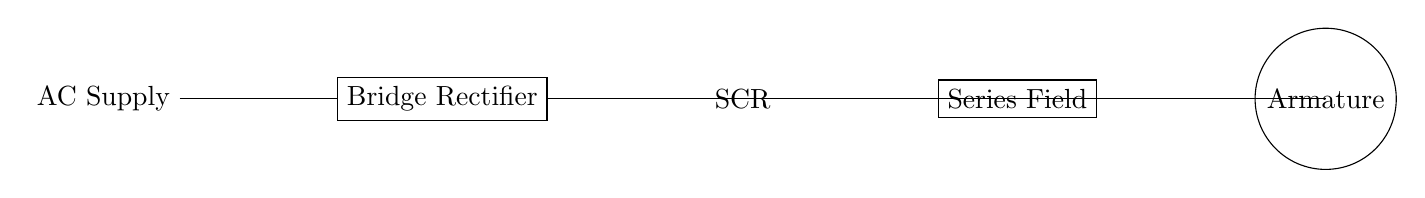
\begin{tikzpicture}[auto, node distance=2cm]
    \node (AC) {AC Supply};
    \node [right=of AC, draw] (BR) {Bridge Rectifier};
    \node [right=of BR] (SCR) {SCR};
    \node [right=of SCR, draw] (SF) {Series Field};
    \node [right=of SF, draw, circle] (A) {Armature};
    
    \draw (AC) -- (BR);
    \draw (BR) -- (SCR) -- (SF) -- (A);
    \draw (A) |- (BR);
\end{tikzpicture}
\captionof{figure}{DC Series Motor Speed Control}
\end{center}

\begin{itemize}
    \item Bridge rectifier converts AC to DC.
    \item SCR controls average voltage to motor.
    \item Firing angle controlled by potentiometer.
    \item Series field and armature current is the same.
\end{itemize}
\end{solutionbox}

\begin{mnemonicbox}
\mnemonic{SCRAM: SCR Controls Rectified Armature and Motor speed.}
\end{mnemonicbox}

\questionmarks{5(c OR)}{7}{Explain construction, working of Stepper motor Give and its applications}

\begin{solutionbox}
Stepper motor is an electromechanical device that converts electrical pulses into discrete mechanical movements.

\textbf{Construction:}
\begin{itemize}
    \item \keyword{Stator}: Contains multiple coil windings arranged in phases.
    \item \keyword{Rotor}: Permanent magnet or soft iron (reluctance type).
    \item \keyword{Bearings}: Support shaft and allow rotation.
\end{itemize}

\textbf{Applications:}
\begin{itemize}
    \item CNC machines and 3D printers.
    \item Robotics and automation.
    \item Medical equipment.
    \item Office equipment (printers, scanners).
\end{itemize}
\end{solutionbox}

\begin{mnemonicbox}
\mnemonic{REACT: Rotation Exactly At Controlled Timing.}
\end{mnemonicbox}

\end{document}
